\documentclass{beamer}
\usepackage{subfig}
\usepackage{amsmath}
\usepackage{bm}

\DeclareMathOperator*{\argmax}{arg\,max}
\DeclareMathOperator*{\argmin}{arg\,min}


\title{Model Selection and Bias-Variance tradeoff}
\author{Prof. Alessandro Lucantonio}
\institute{Aarhus University - Department of Mechanical and Production Engineering}
\date{?/?/2023}

\begin{document}
	\frame{\titlepage}
	
	\begin{frame}
		\frametitle{Motivations - Training vs test error}
		\begin{figure}
			\centering
			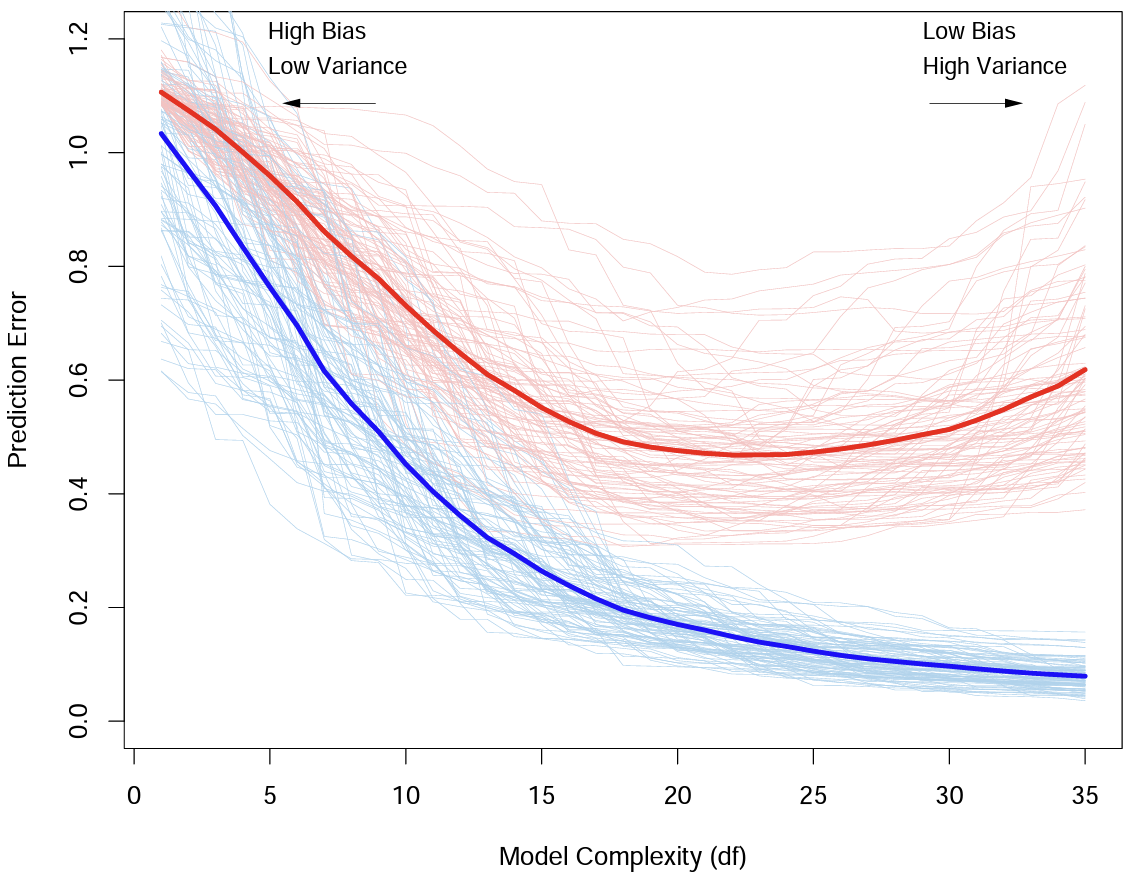
\includegraphics[scale=0.8]{images/model_selection_general_idea}
			\caption{Training (blue) vs text (red) error as the model complexity varies.}
		\end{figure}
	\end{frame}
	
	\begin{frame}
		\frametitle{Motivations - general idea}
		ML in one word: \textbf{generalization}!
		
		\vspace{5mm}
		
		Recall that we have to find a balance between fitting, on training data, and model complexity. Even though we limit the complexity of our model, training set does not provide a good estimate of test error.
		
		\vspace{5mm}
		
		In other words, generalization is compromised if we choose hyperparameters according to (only) training error.
	\end{frame}

	\begin{frame}
		\frametitle{Model selection and model assessment}
		Model selection: estimate the performance of different models trained with different hyperparameters. 
		
		\vspace{5mm}
		
		Model assessment: after choosing a final model we evaluate its perfomance on \textsl{completely new} test data.
		
		\vspace{5mm}
		
		N.B. Model selection and model assessment must be kept separated. Once we have chosen a final model, we are done with the model selection phase and model assessment is needed only to test the model on new data.
	\end{frame}

\end{document}